%\documentclass[final,leqno,onefignum,onetabnum]{siamltexmm}
\documentclass[]{article}
\usepackage{amsmath}
\usepackage{paralist}
\usepackage{amssymb}
\usepackage{subcaption}

\usepackage{graphicx} % Allows including images

\title{An application of Spectral Clustering on Named Entity Recognition}

\author{Ali Josue Limon; Michele Cer\'u \\ 
	\texttt{ajl649@nyu.edu }; \texttt{mc3784@nyu.edu}
}
\begin{document}
	\maketitle
	\newcommand{\slugmaster}{%
		\slugger{siads}{xxxx}{xx}{x}{x---x}}%slugger should be set to juq, siads, sifin, or siims
	
	
	%\newcommand{\slugmaster}{
	%\slugger{siads}{xxxx}{xx}{x}{x---x}}%slugger should be set to juq, siads, sifin, or siims
	
	\begin{abstract}
		This study explores the peformance of spectral clustering in a Spanish Named Entity Recognition (NER) task. Our approach comprises two main steps. Firstly, we represent each Entity in two different ways: 1) by the embedding vector formed from the entity and 2) by the embedding vector formed from the context and the entity.  Then, we use spectral clustering over the words embeddings  to analyze weather the words cluster according to their labels or not.  In order to train the word embedding, we used Word2Vec algorithm over a huge Spanish Corpus with the skip-gram and CBOW models. Our results suggest that this approach performs better than the standard k-means cluster. However, the clustering accuracy is still very low and this suggests that spectral clustering applied on word embedding is not by itself enough to solve the NER task. 
		
	\end{abstract}
	
	\section{Introduction}
	
	Named Entity Recognition (NER) is one of the important parts of NLP. It aims to find and classify expressions of special meaning in texts written in natural language.  These expressions can belong to different predefined classes such as Person, Organization and Location. 
	
	The main algorithms that are currently used for NER in English involves Neural Networks that are trained in a supervised way using large corpuses of labeled data. However, in most languages and domains, there is only a very small amount of supervised training data available, and consequently supervised algorithms are hard to train. Specifically for Spanish, NER is a challenging problem because of the lack of resources and labeled data. Compared with supervised and semi-supervised methods, unsupervised approach for entity recognition can overcome the difficulties on requirement of a large amount of labeled data. 
	
	In this paper we investigate whether spectral clustering techniques can be successfully applied to NER in Spanish. In order to do so, we transform the original input, defined by the the word2Vector embeddings of entities and context, into a set of orthogonal eigenvectors. Then, We work in the space defined by the first few eigenvectors, using standard clustering techniques in the reduced space.
	
	The paper is organized as follows. In Section 2, we provide a explanation of the data used to accomplish the study. Section 3 describes the architecture to create the word embeddings. Section 4 presents our framework for NER and Section 5 explains the metric used to evaluate results. In Section 6 the experiments and results are discussed.  Finally, Section 7 presents the conclusions.
	
	\section{Data}
	The experimentation of this work will be carried on a corpora that consist of sentences extracted from news articles. The corpora corresponds to the \emph{CoNLL 2002} Shared Task Spanish data, the original source being the \emph{EFE Spanish Newswire Agency}.  The data consists of two columns separated by a single space. The first item on each line is a word and the second the named entity tag. In this dataset, there are four types of entities: person names (PER), organizations (ORG), locations (LOC) and miscellaneous names (MISC) and other (O). This dataset contains 11,752 sentences, 369,171 words and 26,706 Name Entities.  
	
	In order to create the word embedding, we added to the \emph{CoNLL 2002} dataset an unannotated corpus of the Spanish Billion Words Corpus [reference] with a total of 1,420,665,810 raw words,  46,925,295 sentences and 3,817,833 unique tokens. Both Corpuses are preprocessed by replacing all non-alphanumeric characters with whitespaces, all numbers with the token ''DIGITO'' and all the multiple whitespaces with only one whitespace.
	
	
	
	\section{Word2Vector Embedding}
	
	Word2vec is a two-layer neural net that processes text. Its input is a text corpus and its output is a set of vectors: feature vectors for words in that corpus. 
	
	The purpose and usefulness of Word2vec is to group the vectors of similar words together in vectorspace. That is, it detects similarities mathematically. Word2vec creates vectors that are distributed numerical representations of word features, features such as the context of individual words. It does so without human intervention. 
	
	Word2Vec works in two ways, either using context to predict a target word (a method known as continuous bag of words, or CBOW), or using a word to predict a target context, which is called skip-gram. For both approaches a neural network is trained with a single hidden layer to perform a certain task depending of the approach. 
	
	\begin{figure}
		\begin{subfigure}{.5\textwidth}
			\centering
			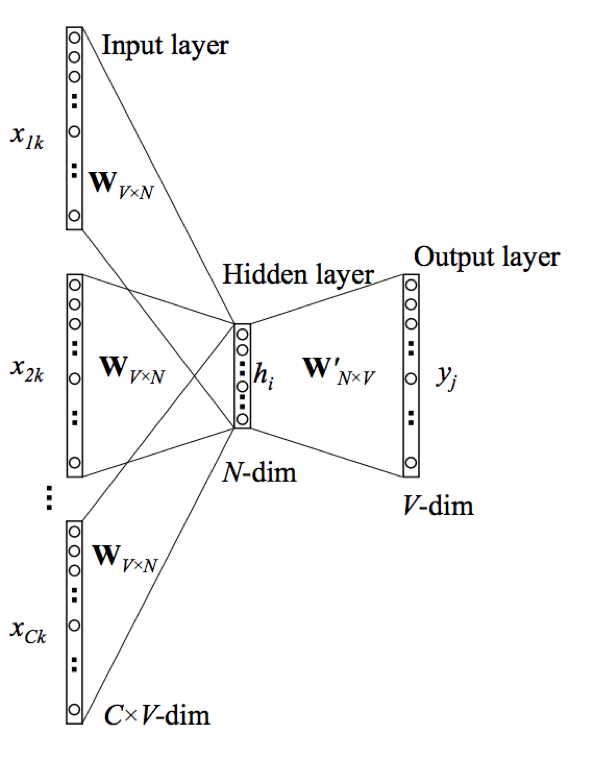
\includegraphics[width=.8\linewidth]{Figures/CBOW}
			\caption{CBOW}
			\label{fig:sfig1}
		\end{subfigure}%
		\begin{subfigure}{.5\textwidth}
			\centering
			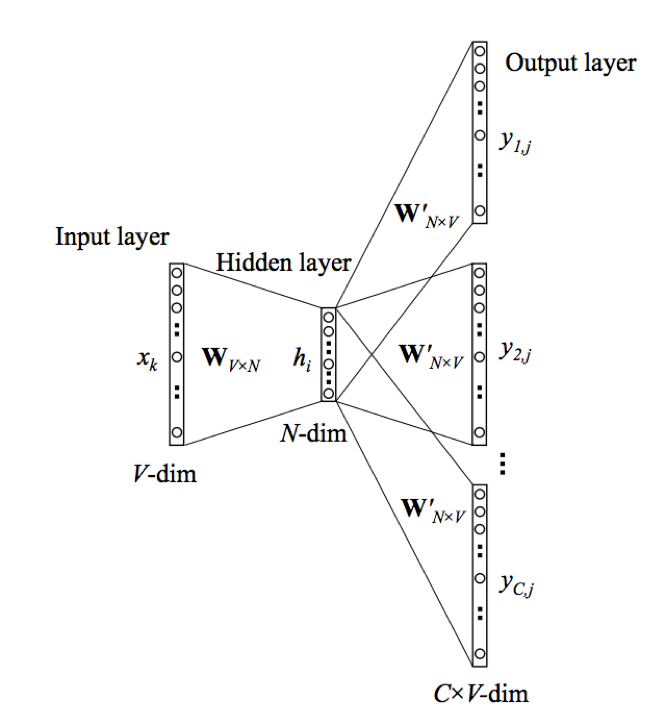
\includegraphics[width=.8\linewidth]{Figures/Skip}
			\caption{Skip-gram}
			\label{fig:sfig2}
		\end{subfigure}
		\caption{Word2Vector Algorithm}
		\label{fig:fig}
	\end{figure}
	
	\section{Problem Formulation}
	Our first goal is to estimate a vector for each entity that captures a large number of precise syntactic and semantic word relationships. For this purpose, we creat an embedding matrix, which will transform the entity's words into a dense word embedding.  To do so, we make use of a simple one-hot vector that represent every word as an $\mathbb{R}^{|V|}$ vector with all 0s and one 1 at the index of that word in the $|V|$ vocabulary created by the embedding Figure \ref{fig:DE}.
	
	\begin{figure}[h]
		\caption{Dense Word Embedding}
		\centering
		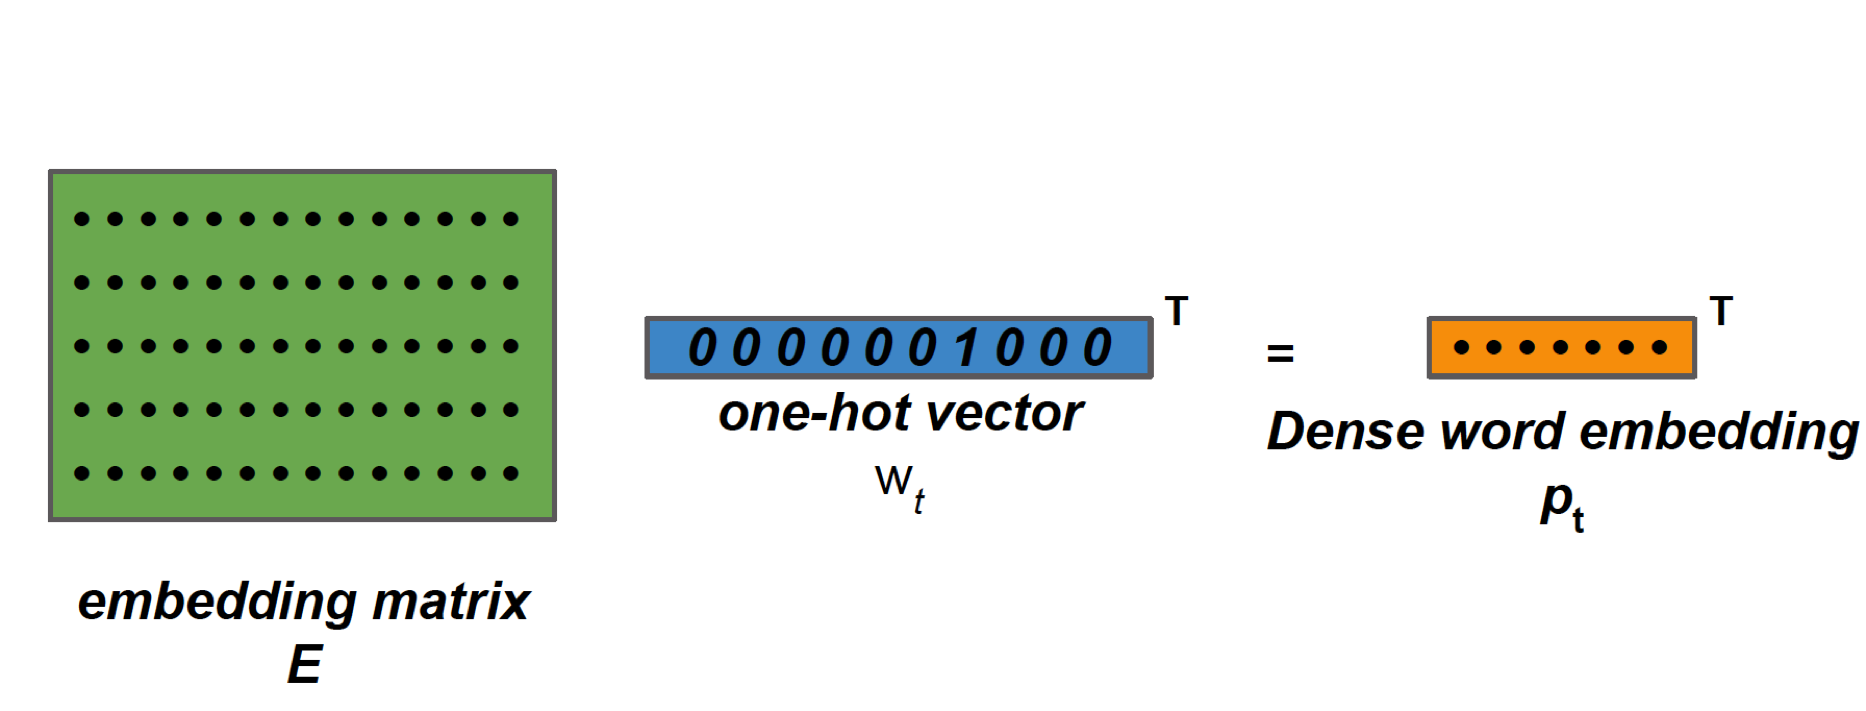
\includegraphics[width=1\textwidth]{Figures/Embeddings}
		\label{fig:DE}
	\end{figure}
	
	
	In this work, each entity can be represented in two different ways. The first one takes into account the embedding of the entity and the second, in addition to the entity, incorporates the embedding of the surrounded words (context). As each entity can be composed by one or more words, we use the average of the embeddings for each word to create the final entity embedding. Figures \ref{fig:gull} shows the two approaches used to compute the final entity embedding.  
	
	

	\begin{figure}[h]
		\caption{Entity embedding under both approaches }
		\centering
		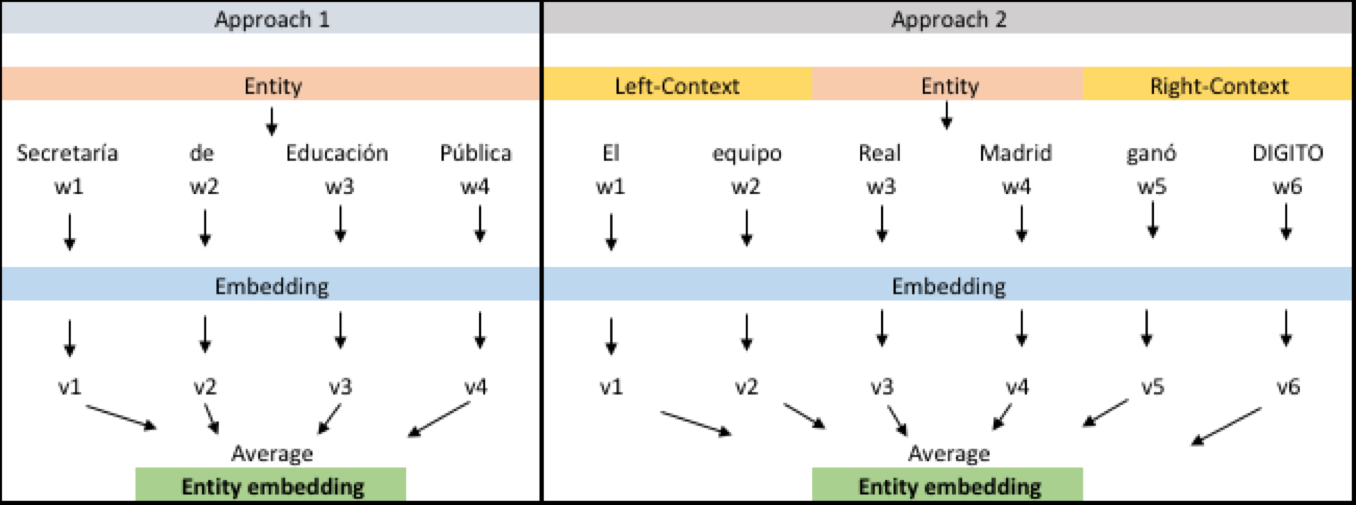
\includegraphics[width=0.9\textwidth]{Figures/EntityEmb}
		\label{fig:gull}
	\end{figure}
	
	Finally, the clustering is done using spectral cluster algorithm on the entity embeddings. Results are compared using skip-gram and CBOW algorithms for the word embeddings and using different kernels for the spectral clustering. 
	
	
	
	\section{Evaluation}
	To compare the different models we ran, we used the Adjusted Rand index \cite{rand},  that evaluate the accuracy of the predicted labels of the clustering given the ground truth of the label. 
	This index looks at each pair of sample, and evaluate the consistency of the prediction given the true label. Calling $C$ the ground truth clustering and $C'$ the predicted one, there are four possible set of pairs:
	$$
	\begin{array}{ll}
	S_{11} = \{\text{pairs belonging to the same cluster both in C and C'} \}\\
	S_{00} =  \{\text{pairs belonging to different cluster both in C and C'} \}\\
	S_{10} =  \{\text{pairs belonging to the same cluster both C but to different ones in C'} \}\\
	S_{01} =  \{\text{pairs belonging to the same cluster both C' but to different ones in C} \}\\
	\end{array}
	$$
	Calling with $n_{11}$ the number of sample in the first set (and analogously for the other sets), the Rand index is defined as:
	$$
	R=\frac{n_{11}+n_{00}}{n_{11}+n_{10}+n_{01}+n_{00}} = \frac{n_{11}+n_{00}}{{ n\choose 2}}
	$$
	where $n$ is the total number of sample. This index range from 0 (when C and C' don't agree on any pair of points) and 1 (when C and C' agree on every pairs). The Adjusted Rand index is defined by rescaling it considering the value that a random clustering would have, doing so the index value is 0 for random clusters. 
	
	\section{Experiments and Discussion}

%\begin{itemize}  \label{confusion} 
%	\item Size of the word  embedding space: $d_E$.
%	\item Technique used for the word embedding training: cbow  or skip-gram.
%	\item Number of words embedding considered around the target word: $n_w$.
%	\item Kernell used for the spectral clustering:
%	\begin{enumerate}
%		\item Cosine similarity 
%		\item Knearest neighbours 
%		\item $k(x,y)=exp(-\gamma ||x-y||_1)$
%	\end{enumerate} 
%\end{itemize}  

\begin{figure}[h]
	\caption{Parameters used to train the model}
	\centering
	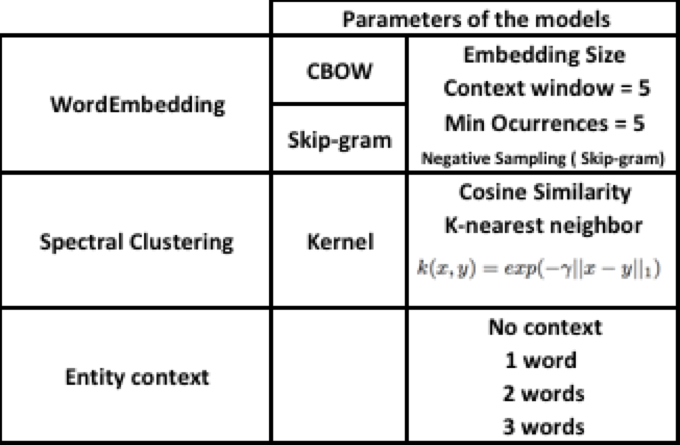
\includegraphics[width=0.6\textwidth]{Figures_Mik/Parameters.png}
	\label{fig:gull}
\end{figure}


After Training the model with different combination of parameters, we found that the best model is the one that uses a CBOW embedding with dimension size $d_E=100$, average over $n_w=3$ entity context words, and the cosine similarity as the kernel for spectral clustering. The spectral clustering has also a comparable Rand index value for small values of $\gamma$. In the plot we reported the results for this two model compared with the Rand index obtained applying k-means clustering to the embedding vectors. 

	\begin{figure}\label{fig:best}
	\centering
	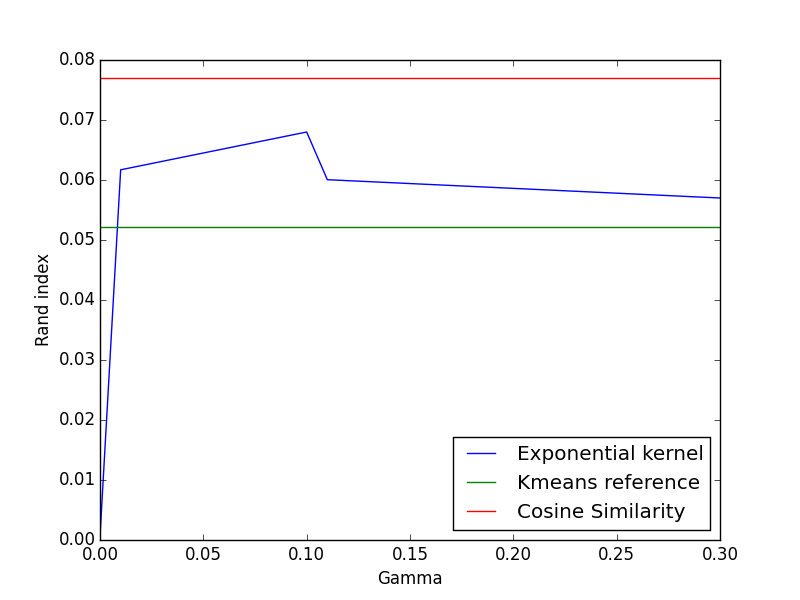
\includegraphics[width=0.8\textwidth]{Figures_Mik/results.png} 
	\caption{The blue line show the rand index for the  exponential kernel model trained for different value of $\gamma$. The red line is the best model (cosine similarity) and the green line is the kmeans clustering, reported here as a bench mark } 
\end{figure}
The following table contains the correspondence between the numeric label used for the clusters and its name entity, if also contain the total number of samples for each clusters: 
\begin{center}
	\begin{tabular}{ |c|c|c|} 
		\hline
		Cluster Label & Name Entity & Samples\\
		\hline
	0 & Organization & 7953\\
		\hline
1 & Location & 4743\\
		\hline
 2 & Person & 5314\\
		\hline
 3 & Miscellaneous & 2441\\
		\hline
	\end{tabular}
\end{center}
The figures with the confusion matrices describe how the three model described here (Kmeans, Spectral with exponential kernel and Spectral with Cosine similarity) compere with an ideal perfect clustering. We notice that the worst cluster in every models is the number 3 that correspond with the named entity "Miscellaneous" that is an ambiguous label and therefore it is reasonable that it is not actually possible to obtain a cluster for it.
	
	
	\begin{figure}
		\label{confusion} 
		\begin{minipage}[b]{0.5\linewidth}
			\centering
			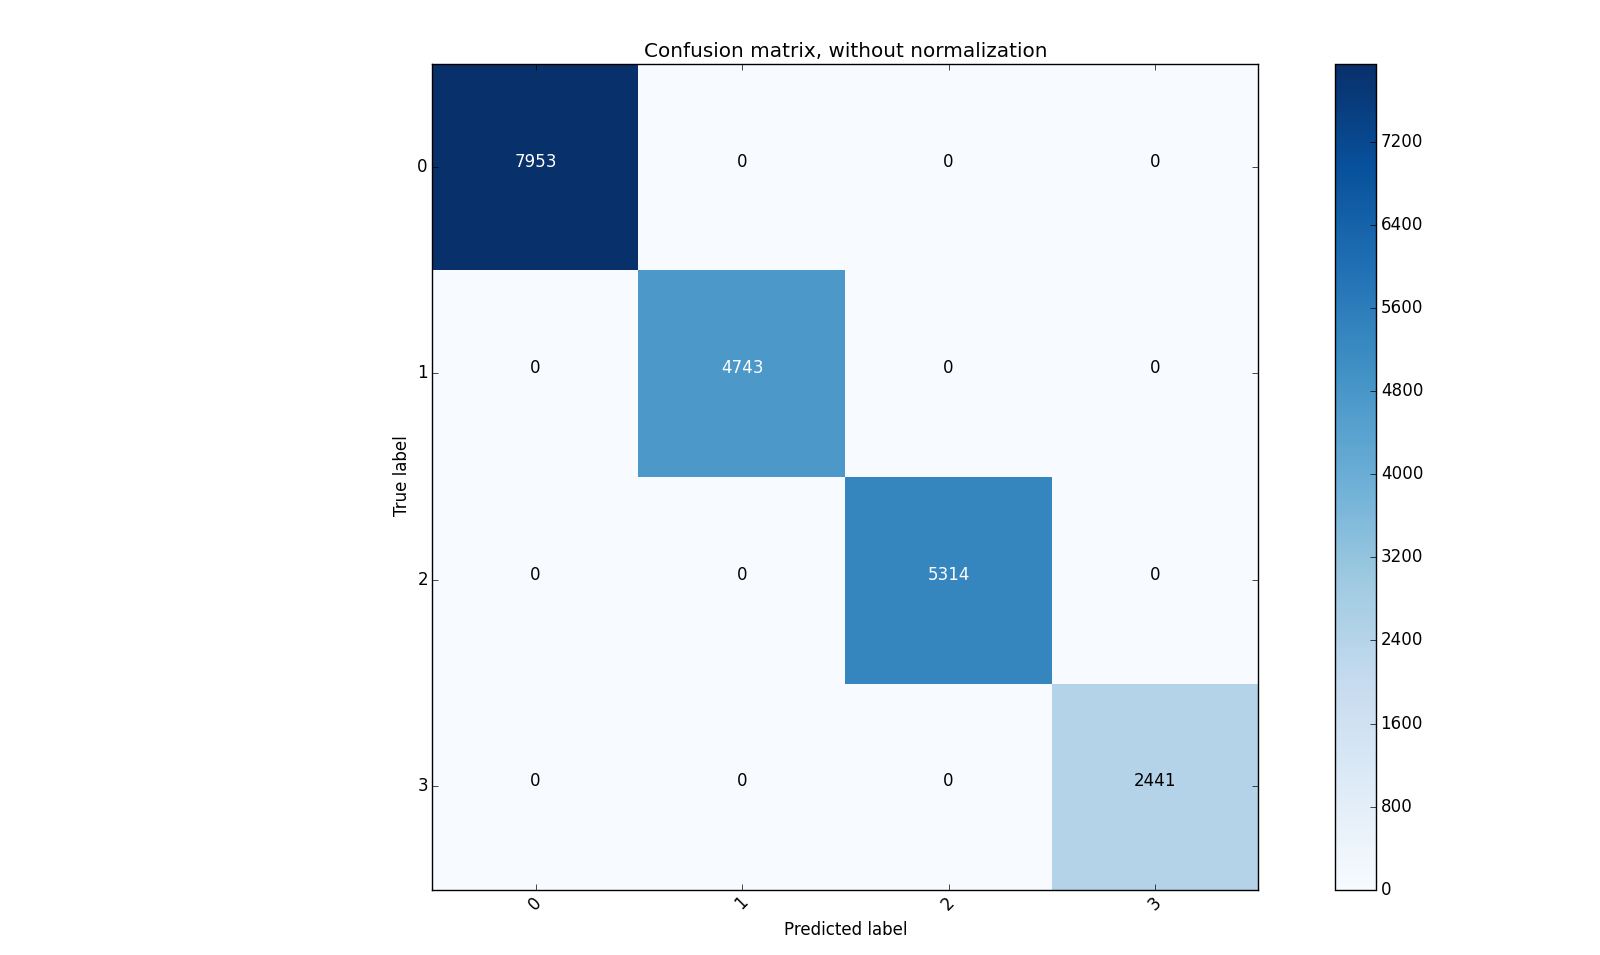
\includegraphics[width=1\linewidth]{Figures_Mik/label_distribution.png} 
			\caption{True label distribution} 
			\vspace{4ex}
		\end{minipage}%%
		\begin{minipage}[b]{0.5\linewidth}
			\centering
			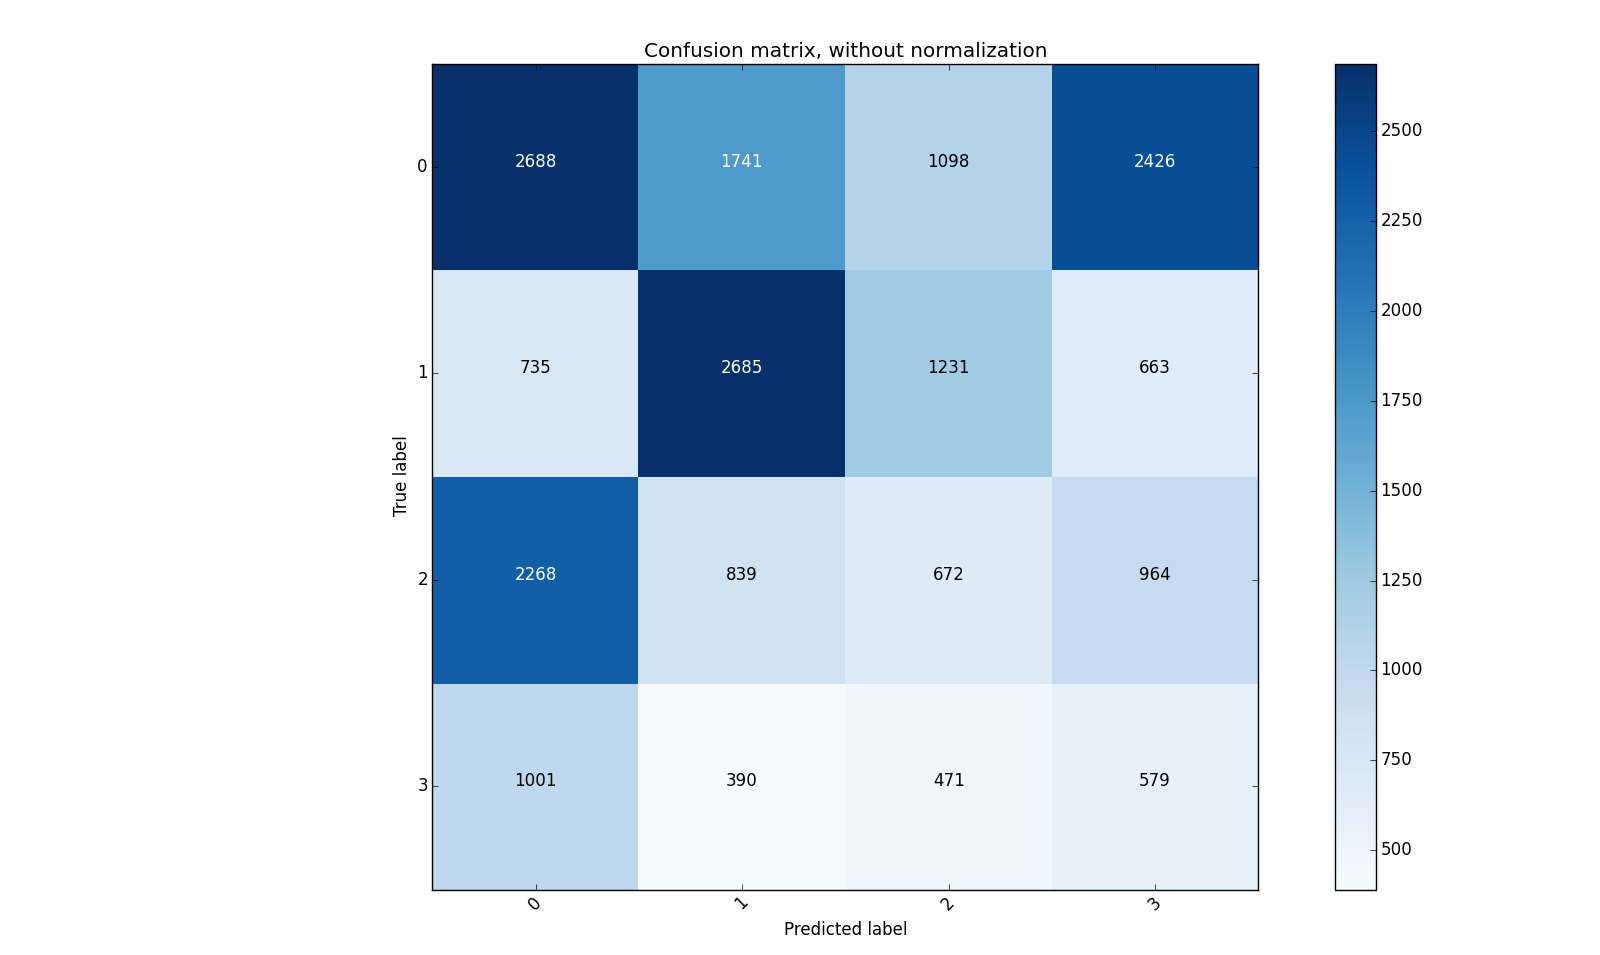
\includegraphics[width=1\linewidth]{Figures_Mik/kmeans2.png} 
			\caption{Kmeans Clustering} 
			\vspace{4ex}
		\end{minipage} 
		\begin{minipage}[b]{0.5\linewidth}
			\centering
			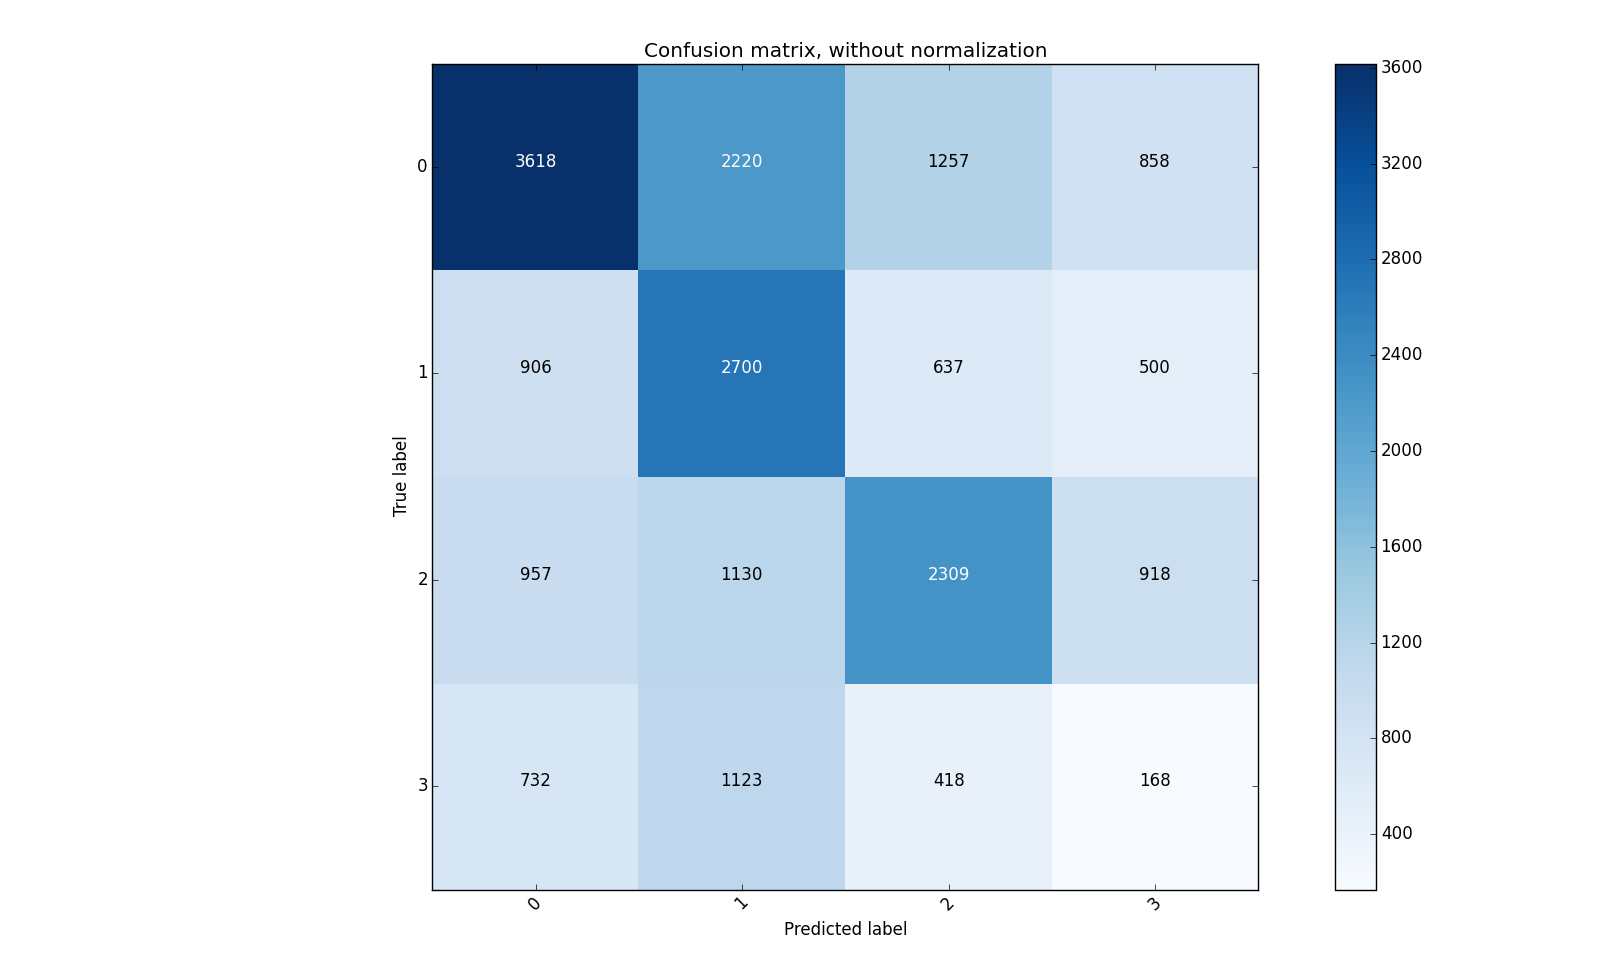
\includegraphics[width=1\linewidth]{Figures_Mik/bestModel2.png} 
			\caption{Spectral(exponential kernel)} 
			\vspace{4ex}
		\end{minipage}%% 
		\begin{minipage}[b]{0.5\linewidth}
			\centering
			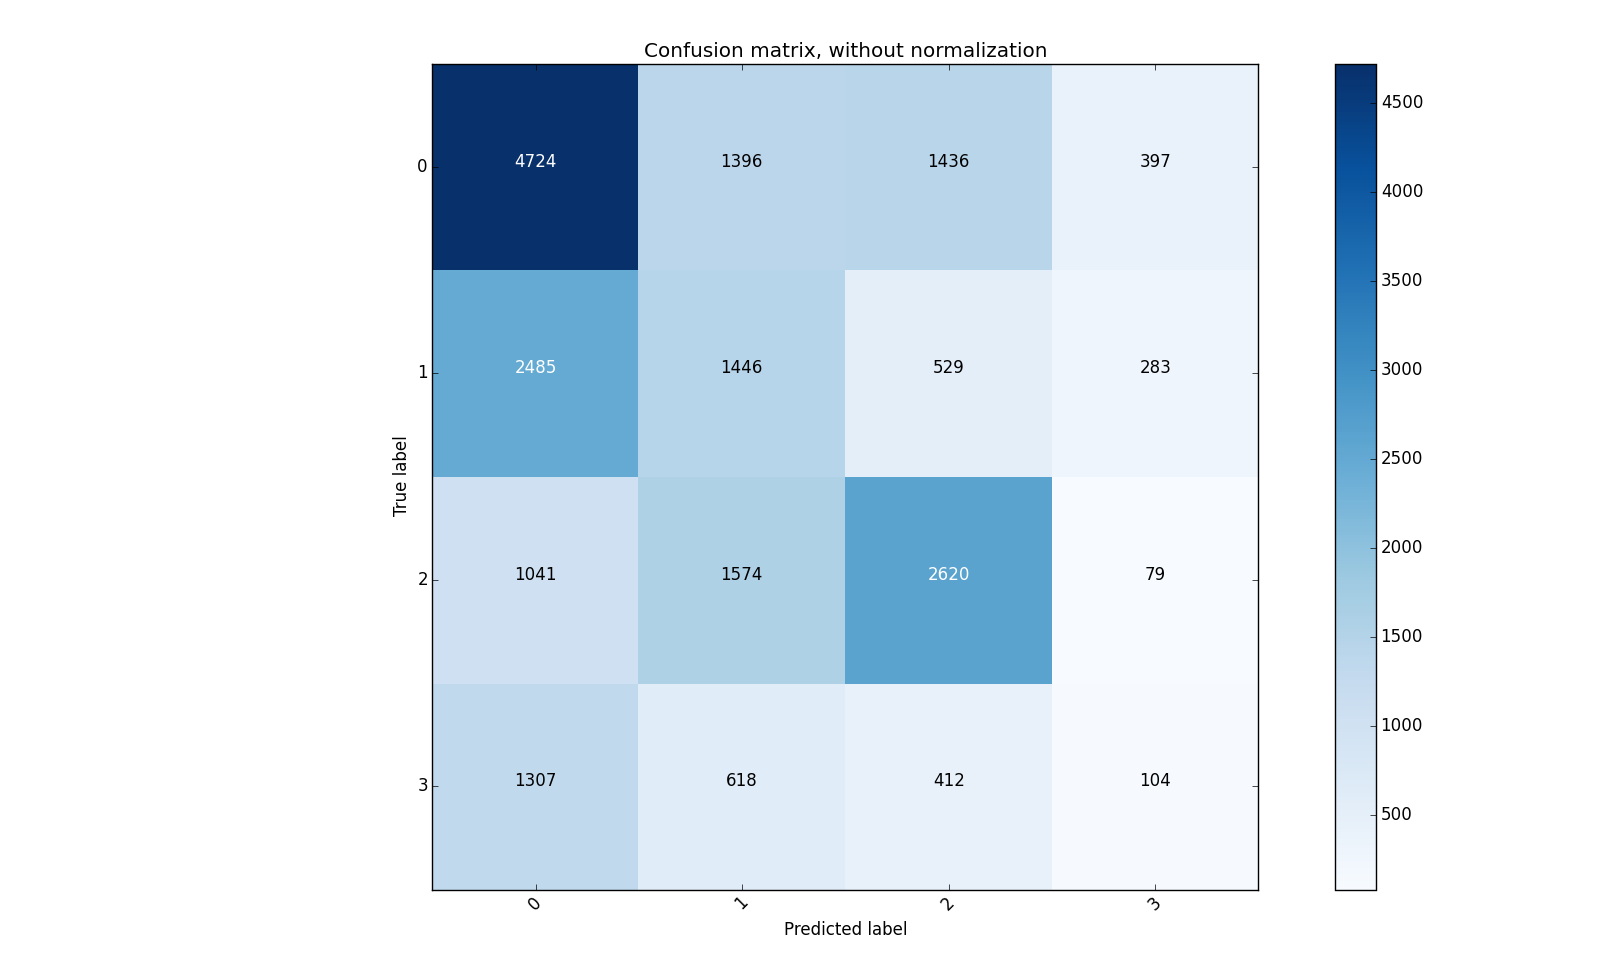
\includegraphics[width=1\linewidth]{Figures_Mik/cosSimConfMat2.png} 
			\caption{Spectral(Cosine similarity)} 
			\vspace{4ex}
		\end{minipage} 
	\end{figure}
	
	
	\section{Conclusions}
	This paper presents a technique for Named Entity Recognition using spectral clustering and word embeddings. The main conclusion given the results is that our approach does not seem to perform very well creating clusters according to the named entities labels. This could be due to the fact that word embeddings representation encloses many different properties of the language, and named entity it is just one of them, consequently it is not possible to achieve a very good cut of the cluster according just to the named entities labels. We feel that with more tunning of parameters could achieve slightly better results. However, we do not think that this alone can be the solution of the problem. 
	
	
	

	
	\pagestyle{myheadings}
	\thispagestyle{plain}
	
	
	\begin{thebibliography}{1}
		\bibitem{dataset} http://www.cnts.ua.ac.be/conll2002/ner/
		\bibitem{spectral}http://www.cims.nyu.edu/$\sim$bandeira/TenLecturesFortyTwoProblems.pdf
		\bibitem{popescu} Popescu, M., \& Hristea, F. (2011). State of the art versus classical clustering for unsupervised word sense disambiguation. Artificial Intelligence Review, 35(3), 241?264. http://dx.doi.org/10.1007/s10462-010-9193-7.  
		\bibitem{vecSp} http://crscardellino.me/SBWCE/
		\bibitem{word2vec} Mikolov, T., Chen, K., Corrado, G., \& Dean, J. (2013). Efficient Estimation of Word Representations in Vector Space. arXiv preprint arXiv:1301.3781. 
		\bibitem{rand}Rand, William M.: Objective Criteria for the Evaluation of Clustering Methods. Journal of the American Statistical Association, 66(336):846? 850, 1971.
	\end{thebibliography} 
	
	
\end{document}